\documentclass[aspectratio=169,10pt]{beamer}
\usepackage[T1]{fontenc}
\usepackage{amsmath,amssymb,amsfonts}
\usepackage{bm}
\usepackage{tikz}
\usepackage{xcolor}
\usetikzlibrary{arrows.meta,positioning,shapes,calc}

\definecolor{parchment}{HTML}{F4E8C8}
\definecolor{paper}{HTML}{FAF1D8}
\definecolor{ink}{HTML}{1A1A1A}
\definecolor{inkgray}{HTML}{5A5A5A}
\definecolor{accentred}{HTML}{8B1A1A}
\definecolor{accentgreen}{HTML}{2D5F2C}
\definecolor{accentblue}{HTML}{1F4E79}
\definecolor{redbg}{HTML}{F7E0DE}
\definecolor{grnbg}{HTML}{E0EBDC}
\definecolor{blubg}{HTML}{DDE6EF}
\definecolor{labelbg}{HTML}{EFE0B0}

\usefonttheme{serif}
\setbeamercolor{background canvas}{bg=parchment}
\setbeamercolor{normal text}{fg=ink}
\setbeamercolor{structure}{fg=ink}
\setbeamercolor{frametitle}{fg=ink,bg=parchment}
\setbeamercolor{title}{fg=ink}
\setbeamercolor{itemize item}{fg=ink}
\setbeamercolor{itemize subitem}{fg=ink}
\setbeamercolor{item}{fg=ink}
\setbeamercolor{caption name}{fg=ink}
\setbeamertemplate{navigation symbols}{}
\setbeamertemplate{itemize item}{\textbullet}

\setbeamertemplate{frametitle}{%
  \vspace{0.30em}%
  \begin{center}%
    {\bfseries\Large\insertframetitle\par}%
    \vspace{0.28em}%
    {\color{ink}\rule{0.86\paperwidth}{0.4pt}}%
  \end{center}%
  \vspace{0.10em}%
}
\setbeamertemplate{footline}{%
  \hbox to \paperwidth{\hfil\itshape\small\insertframenumber\hspace{0.7em}}%
  \vspace{0.35em}%
}

\newcommand{\vY}{\bm{Y}}
\newcommand{\vy}{\bm{y}}
\newcommand{\vA}{\bm{A}}
\newcommand{\vB}{\bm{B}}
\newcommand{\valpha}{\bm{\alpha}}
\newcommand{\vn}{\bm{n}}
\newcommand{\vs}{\bm{s}}
\newcommand{\vW}{\bm{W}}
\newcommand{\T}{^{\mathsf T}}
\newcommand{\Hh}{^{\mathsf H}}
\newcommand{\norm}[1]{\left\lVert #1\right\rVert}
\DeclareMathOperator*{\argmin}{arg\,min}

\tikzset{
  flowbox/.style={draw=ink,fill=paper,line width=0.6pt,
                  minimum width=2.5cm,minimum height=1.0cm,
                  align=center,font=\small\bfseries,inner sep=4pt},
  smallbox/.style={draw=ink,fill=paper,line width=0.4pt,
                   minimum width=0.7cm,minimum height=0.55cm,
                   inner sep=2pt,align=center,font=\footnotesize\itshape},
  method/.style={draw=accentgreen,fill=grnbg,line width=1.0pt,
                 align=center,font=\small\bfseries,inner sep=6pt},
  issue/.style={draw=accentred,fill=redbg,line width=1.0pt,
                align=center,font=\small\bfseries,inner sep=6pt},
  idea/.style={draw=accentblue,fill=blubg,line width=1.0pt,
               align=center,font=\small\bfseries,inner sep=6pt},
  flowarr/.style={-{Stealth[length=2.5mm,width=2mm]},line width=0.7pt},
  softarr/.style={-{Stealth[length=2mm,width=1.6mm]},line width=0.5pt,color=inkgray}
}

\newcommand{\bottomnote}[1]{%
  \begin{center}{\itshape\small #1}\end{center}}

\newcommand{\papercover}[4]{%
  \begin{frame}[plain]
    \vfill
    \begin{center}
      {\bfseries\Huge #1\par}
      \vspace{0.8cm}
      {\Large #2\par}
      \vspace{0.35cm}
      {\itshape\large\color{inkgray}#3\par}
      \vspace{0.55cm}
      {\small\texttt{\detokenize{#4}}\par}
    \end{center}
    \vfill
  \end{frame}}

\newcommand{\twocolmodel}[4]{%
  \begin{columns}[T,onlytextwidth]
    \begin{column}{0.48\textwidth}#1\end{column}
    \begin{column}{0.48\textwidth}#2\end{column}
  \end{columns}
  \bottomnote{#3\\#4}}


\usetikzlibrary{decorations.pathreplacing,decorations.pathmorphing,shapes.misc}

\newcommand{\jj}{\mathrm{j}}
\newcommand{\sinc}{\operatorname{sinc}}
\newcommand{\rx}{\mathrm{rx}}
\newcommand{\tx}{\mathrm{tx}}
\newcommand{\diag}{\mathrm{diag}}

% ===== visual helpers used only in this deck =====
\tikzset{
  stepbadge/.style={
    draw=ink, fill=labelbg, line width=0.6pt, circle,
    inner sep=0pt, minimum size=0.85cm,
    font=\bfseries\small
  },
  notecard/.style={
    draw=ink, fill=paper, line width=0.5pt, rounded corners=2pt,
    align=center, inner sep=5pt, font=\small
  },
  greencard/.style={
    draw=accentgreen, fill=grnbg, line width=0.8pt, rounded corners=2pt,
    align=center, inner sep=5pt, font=\small
  },
  redcard/.style={
    draw=accentred, fill=redbg, line width=0.8pt, rounded corners=2pt,
    align=center, inner sep=5pt, font=\small
  },
  bluecard/.style={
    draw=accentblue, fill=blubg, line width=0.8pt, rounded corners=2pt,
    align=center, inner sep=5pt, font=\small
  },
  thinkbubble/.style={
    draw=accentblue, fill=blubg!75, line width=0.6pt,
    rounded corners=6pt, align=center, inner sep=6pt,
    font=\itshape\small
  },
  tinybox/.style={
    draw=ink, fill=paper, line width=0.4pt, rounded corners=1pt,
    align=center, inner sep=3pt, font=\scriptsize
  },
  brace/.style={decorate, decoration={brace, amplitude=4pt, raise=2pt}, line width=0.55pt, color=inkgray}
}

% Step badge sits BELOW the title rule (the rule is around 1.4cm from page top
% in this 16:9 deck). 0.62cm badge + a one-line caption to the right.
\newcommand{\stepbadgehdr}[2]{%
  \begin{tikzpicture}[remember picture,overlay]
    \node[stepbadge,anchor=north west,minimum size=0.62cm,font=\bfseries\footnotesize]
      at ([xshift=0.30cm,yshift=-1.62cm]current page.north west) {#1};
    \node[anchor=west,font=\scriptsize\itshape\color{inkgray}]
      at ([xshift=1.00cm,yshift=-1.92cm]current page.north west) {#2};
  \end{tikzpicture}%
}

\begin{document}

% =====================================================================
% Cover
% =====================================================================
\begin{frame}[plain]
  \vspace{0.6cm}
  \begin{center}
    {\bfseries\Huge How ICI Forms\par}
    \vspace{0.20cm}
    {\Large\itshape Doppler, OFDM, and the loop that does not quite close\par}

    \vspace{0.55cm}
    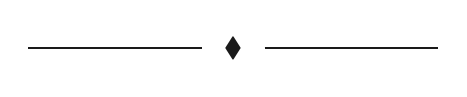
\begin{tikzpicture}
      \draw[ink,line width=0.5pt] (-2.6,0) -- (-0.4,0);
      \node at (0,0) {\color{ink}$\blacklozenge$};
      \draw[ink,line width=0.5pt] (0.4,0) -- (2.6,0);
    \end{tikzpicture}
    \vspace{0.45cm}

    % Hero illustration: clean carrier comb -> Doppler skew -> partial-FFT recovery
    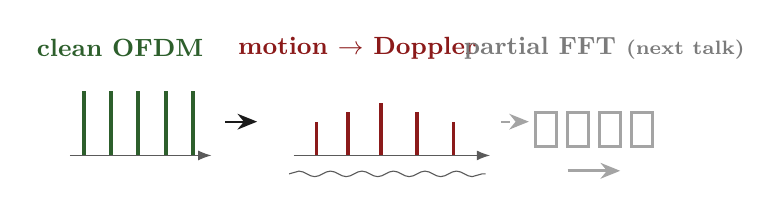
\begin{tikzpicture}[x=0.58cm,y=0.78cm,>=Latex]
      % left: clean comb
      \node[font=\small\bfseries\color{accentgreen}] at (-5.4,1.55) {clean OFDM};
      \foreach \x in {-6.2,-5.6,-5.0,-4.4,-3.8} {
        \draw[accentgreen,line width=1.4pt] (\x,-0.2) -- (\x,0.85);
      }
      \draw[inkgray,->] (-6.5,-0.2) -- (-3.4,-0.2);

      \node[font=\small\bfseries\color{accentred}] at (-0.2,1.55) {motion $\to$ Doppler};
      \foreach \x/\h in {-1.10/0.55,-0.42/0.70,0.32/0.85,1.10/0.70,1.90/0.55} {
        \draw[accentred,line width=1.4pt] (\x,-0.2) -- (\x,{-0.2+\h});
      }
      % "wind" wiggle behind
      \draw[inkgray,decorate,decoration={snake,amplitude=1.0pt,segment length=4mm}]
        (-1.7,-0.5) -- (2.6,-0.5);
      \draw[inkgray,->] (-1.6,-0.2) -- (2.7,-0.2);

      \node[font=\small\bfseries\color{inkgray!80}] at (5.2,1.55) {partial FFT \scriptsize(next talk)};
      % four short windows -> one big arrow (greyed: the sequel, not today)
      \foreach \x in {3.7,4.4,5.1,5.8} {
        \draw[inkgray!55,line width=1.0pt] (\x,-0.05) rectangle ++(0.45,0.55);
      }
      \draw[flowarr,color=inkgray!55,line width=1.0pt] (4.4,-0.45) -- (5.55,-0.45);

      % connecting arrows
      \draw[flowarr,color=ink] (-3.10,0.35) -- (-2.40,0.35);
      \draw[flowarr,color=inkgray!55,dashed] (2.95,0.35) -- (3.55,0.35);
    \end{tikzpicture}

    \vspace{0.65cm}
    {\itshape\small\color{inkgray}Part I of the OFDM Doppler workbench: closed loops separate carriers; unfinished loops create leakage\par}
  \end{center}
\end{frame}
% =====================================================================
% Roadmap
% =====================================================================
\begin{frame}{The story in four moves}
\small
\begin{center}
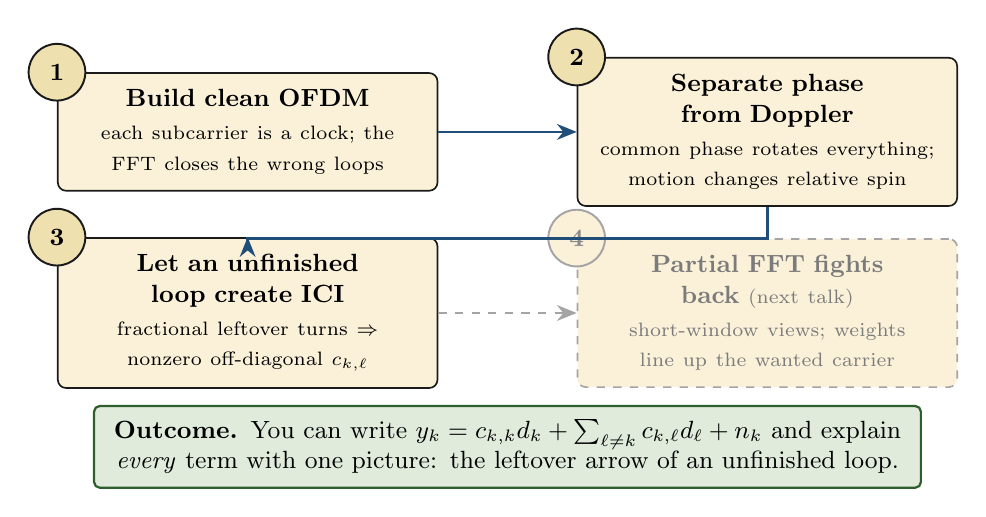
\begin{tikzpicture}[x=1.0cm,y=1.0cm,>=Latex,
   roadcard/.style={draw=ink, fill=paper, line width=0.6pt,
                    rounded corners=3pt, align=center, inner sep=6pt,
                    text width=4.4cm, minimum height=1.35cm, font=\small},
   ghostcard/.style={draw=inkgray!55, fill=paper, line width=0.6pt, dashed,
                    rounded corners=3pt, align=center, inner sep=6pt,
                    text width=4.4cm, minimum height=1.35cm, font=\small,
                    text=inkgray!80},
   roadbadge/.style={circle, draw=ink, fill=labelbg, line width=0.7pt,
                     minimum size=0.72cm, inner sep=0pt, font=\bfseries\small},
   ghostbadge/.style={circle, draw=inkgray!55, fill=paper, line width=0.7pt,
                     minimum size=0.72cm, inner sep=0pt, font=\bfseries\small,
                     text=inkgray!70}]

  % Top row
  \node[roadcard] (s1) at (-3.3,1.3) {%
    \textbf{Build clean OFDM}\\[0.10em]
    \scriptsize each subcarrier is a clock; the FFT closes the wrong loops};
  \node[roadcard] (s2) at (3.3,1.3) {%
    \textbf{Separate phase from Doppler}\\[0.10em]
    \scriptsize common phase rotates everything; motion changes relative spin};

  % Bottom row
  \node[roadcard] (s3) at (-3.3,-1.0) {%
    \textbf{Let an unfinished loop create ICI}\\[0.10em]
    \scriptsize fractional leftover turns $\Rightarrow$ nonzero off-diagonal $c_{k,\ell}$};
  \node[ghostcard] (s4) at (3.3,-1.0) {%
    \textbf{Partial FFT fights back} {\scriptsize(next talk)}\\[0.10em]
    \scriptsize short-window views; weights line up the wanted carrier};

  % Step badges on top-left corner of each card (outside the card box)
  \node[roadbadge] at (s1.north west) {1};
  \node[roadbadge] at (s2.north west) {2};
  \node[roadbadge] at (s3.north west) {3};
  \node[ghostbadge] at (s4.north west) {4};

  % Curved soft arrows
  \draw[flowarr,color=accentblue,line width=0.9pt] (s1.east) -- (s2.west);
  \draw[flowarr,color=accentblue,line width=0.9pt] (s2.south) -- ($(s2.south) + (0,-0.4)$) -| (s3.north);
  \draw[flowarr,color=inkgray!55,line width=0.9pt,dashed] (s3.east) -- (s4.west);

  % Outcome banner
  \node[greencard,minimum width=10.5cm,text width=10.0cm,font=\small]
    at (0,-2.7) {%
    \textbf{Outcome.} You can write $y_k=c_{k,k}d_k+\sum_{\ell\ne k}c_{k,\ell}d_\ell+n_k$ and explain \emph{every} term with one picture: the leftover arrow of an unfinished loop.};
\end{tikzpicture}
\end{center}

\vspace{-0.18cm}
\begin{center}\scriptsize
  \emph{Closed loop} = no leak; \emph{unfinished loop} = ICI.\quad
  \textcolor{accentgreen}{\textbf{green}}=wanted,\quad
  \textcolor{accentred}{\textbf{red}}=leakage,\quad
  \textcolor{accentblue}{\textbf{blue}}=receiver tool.
\end{center}
\end{frame}
% =====================================================================
% 0b. The full OFDM chain in one picture
% (absorbed from ici_unfinished_loop_mod_demod_slides.tex)
% =====================================================================
\begin{frame}{The full OFDM chain in one picture}
\stepbadgehdr{1}{the pipeline for the whole talk; the loop lives inside the FFT box}
\small
\begin{center}
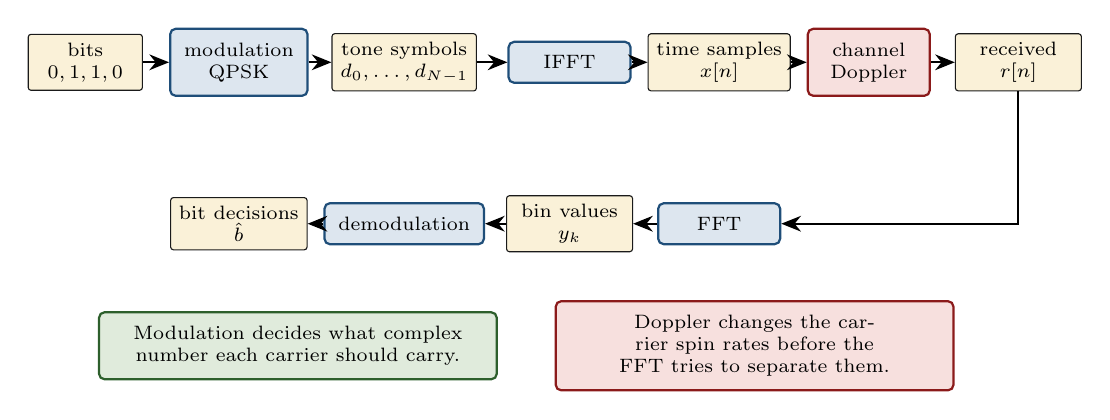
\begin{tikzpicture}[x=1cm,y=1cm,>=Latex]
  \node[tinybox,minimum width=1.45cm] (b) at (-5.6,0.9) {bits\\$0,1,1,0$};
  \node[bluecard,minimum width=1.65cm,font=\scriptsize] (m) at (-3.65,0.9) {modulation\\QPSK};
  \node[tinybox,minimum width=1.75cm] (d) at (-1.55,0.9) {tone symbols\\$d_0,\ldots,d_{N-1}$};
  \node[bluecard,minimum width=1.55cm,font=\scriptsize] (i) at (0.55,0.9) {IFFT};
  \node[tinybox,minimum width=1.60cm] (x) at (2.45,0.9) {time samples\\$x[n]$};
  \node[redcard,minimum width=1.55cm,font=\scriptsize] (ch) at (4.35,0.9) {channel\\Doppler};
  \node[tinybox,minimum width=1.60cm] (r) at (6.25,0.9) {received\\$r[n]$};

  \node[bluecard,minimum width=1.55cm,font=\scriptsize] (f) at (2.45,-1.15) {FFT};
  \node[tinybox,minimum width=1.60cm] (y) at (0.55,-1.15) {bin values\\$y_k$};
  \node[bluecard,minimum width=1.65cm,font=\scriptsize] (dem) at (-1.55,-1.15) {demodulation};
  \node[tinybox,minimum width=1.45cm] (bh) at (-3.65,-1.15) {bit decisions\\$\hat b$};

  \draw[flowarr] (b) -- (m); \draw[flowarr] (m) -- (d); \draw[flowarr] (d) -- (i);
  \draw[flowarr] (i) -- (x); \draw[flowarr] (x) -- (ch); \draw[flowarr] (ch) -- (r);
  \draw[flowarr] (r.south) |- (f.east); \draw[flowarr] (f) -- (y);
  \draw[flowarr] (y) -- (dem); \draw[flowarr] (dem) -- (bh);

  \node[greencard,text width=4.7cm,font=\scriptsize] at (-2.9,-2.70)
    {Modulation decides what complex number each carrier should carry.};
  \node[redcard,text width=4.7cm,font=\scriptsize] at (2.9,-2.70)
    {Doppler changes the carrier spin rates before the FFT tries to separate them.};
\end{tikzpicture}
\end{center}
\bottomnote{Demodulation $=$ de-spin one carrier, then average. Every closed or unfinished loop in this talk lives inside the FFT box; steps 1--3 walk this chain left to right.}
\end{frame}

% =====================================================================
% 1a. Bits to tones
% =====================================================================
\begin{frame}{Start with symbols, not waves}
\stepbadgehdr{1}{name the symbols before they become a waveform}
\small
\begin{columns}[T,onlytextwidth]
  \begin{column}{0.48\textwidth}
    Use an $N=8$ toy OFDM symbol.  Bits are first grouped and mapped to
    constellation points:
    \[
      \begin{array}{c|c|c}
        \text{tone } \ell & \text{bits} & d_\ell\\ \hline
        4 & 10 & -1+\jj\\
        5 & 01 & 1-\jj
      \end{array}
    \]
    \begin{center}\vspace{-0.25cm}
      {\scriptsize\color{inkgray}(QPSK rule: $00\mapsto 1{+}\jj$,\;
       $01\mapsto 1{-}\jj$,\; $10\mapsto -1{+}\jj$,\; $11\mapsto -1{-}\jj$)}
    \end{center}\vspace{-0.15cm}
    Then those symbols are placed into frequency bins:
    \[
      \mathbf d=[d_0,d_1,\ldots,d_7].
    \]
    Later, bin $4$ will be the receiver bin we care about.
  \end{column}
  \begin{column}{0.50\textwidth}
    \begin{center}
    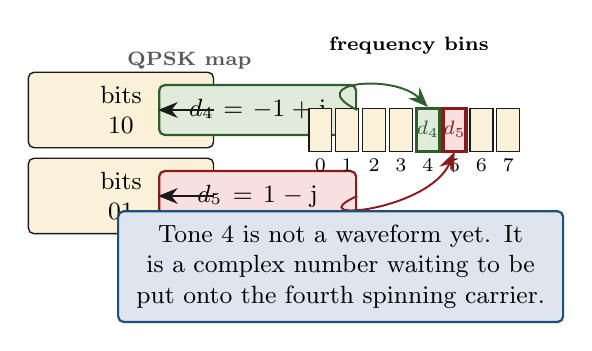
\begin{tikzpicture}[x=0.62cm,y=0.78cm,>=Latex]
      \node[notecard,text width=2.0cm] (b4) at (-3.5,1.2) {bits\\$10$};
      \node[notecard,text width=2.0cm] (b5) at (-3.5,-0.2) {bits\\$01$};
      \node[greencard,text width=2.15cm] (q4) at (-0.7,1.2) {$d_4=-1+\jj$};
      \node[redcard,text width=2.15cm] (q5) at (-0.7,-0.2) {$d_5=1-\jj$};
      \draw[flowarr,color=ink] (b4) -- (q4);
      \draw[flowarr,color=ink] (b5) -- (q5);
      \node[font=\scriptsize\bfseries\color{inkgray}] at (-2.10,2.00) {QPSK map};

      \node[font=\scriptsize\bfseries] at (2.4,2.25) {frequency bins};
      \foreach \i in {0,...,7} {
        \draw[draw=ink,fill=paper,line width=0.45pt] ({0.55*\i+0.35},0.52) rectangle ++(0.47,0.70);
        \node[font=\scriptsize] at ({0.55*\i+0.585},0.30) {\i};
      }
      \draw[draw=accentgreen,line width=1.2pt,fill=grnbg] ({0.55*4+0.35},0.52) rectangle ++(0.47,0.70);
      \draw[draw=accentred,line width=1.2pt,fill=redbg] ({0.55*5+0.35},0.52) rectangle ++(0.47,0.70);
      \node[font=\scriptsize\color{accentgreen}] at ({0.55*4+0.585},0.88) {$d_4$};
      \node[font=\scriptsize\color{accentred}] at ({0.55*5+0.585},0.88) {$d_5$};
      \draw[flowarr,color=accentgreen] (q4.east) .. controls (0.2,1.65) and (2.1,1.80) .. ({0.55*4+0.585},1.25);
      \draw[flowarr,color=accentred] (q5.east) .. controls (0.1,-0.65) and (2.8,-0.45) .. ({0.55*5+0.585},0.52);

      \node[bluecard,text width=5.3cm] at (1.0,-1.35) {%
        Tone $4$ is not a waveform yet. It is a complex number waiting to be put onto the fourth spinning carrier.};
    \end{tikzpicture}
    \end{center}
  \end{column}
\end{columns}
\end{frame}

% =====================================================================
% 1a2. Why carriers exist, and what "modulation" physically does
% (scale example borrowed from juna_slides.tex)
% =====================================================================
\begin{frame}{Why carriers: the channel speaks in waves}
\stepbadgehdr{1}{a wave has two knobs --- height and shift --- and one complex number sets both}
\small
\begin{columns}[T,onlytextwidth]
  \begin{column}{0.48\textwidth}
    \vspace{0.05cm}
    \textbf{Why we need carriers.}
    \begin{itemize}\setlength{\itemsep}{0.30em}
      \item The medium only carries \emph{waves} --- underwater, pressure
        oscillations in a usable band. A transducer cannot launch a raw
        bit train.
      \item A sinusoid is the shape a linear channel \emph{preserves}:
        $f$ in $\to$ $f$ out, only scaled and delayed. It survives the trip.
      \item Different frequencies travel together without mixing and can
        be pulled apart again: each one is a private \emph{lane}.
    \end{itemize}
    \vspace{0.10cm}
    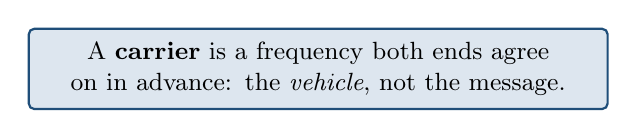
\begin{tikzpicture}
      \node[bluecard,text width=7.0cm] {%
        A \textbf{carrier} is a frequency both ends agree on in advance:
        the \emph{vehicle}, not the message.};
    \end{tikzpicture}
  \end{column}
  \begin{column}{0.50\textwidth}
    \vspace{0.05cm}
    \textbf{How modulation rides one:} the wave's two knobs --- height
    $A$ and shift $\phi$ --- are one complex number $d=A\,e^{\jj\phi}$:
    \[
      A\cos(2\pi f t+\phi)
      \;=\;
      \operatorname{Re}\big\{\,d\,e^{\jj 2\pi f t}\big\}.
    \]
    The QPSK point $d$ \emph{is} the knob pair, re-set once per symbol;
    the math keeps the arrow $d\,e^{\jj 2\pi f t}$.
    \begin{center}
    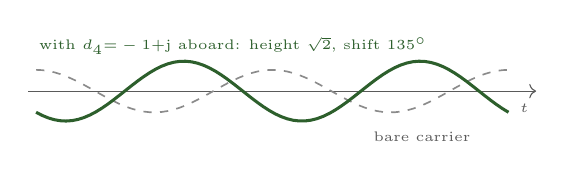
\begin{tikzpicture}[x=1cm,y=1cm]
      \draw[inkgray,->] (-0.1,0) -- (6.35,0);
      \node[font=\tiny\color{inkgray}] at (6.2,-0.22) {$t$};
      \draw[inkgray!70,dashed,line width=0.6pt,domain=0:6.0,samples=80]
        plot (\x,{0.27*cos(120*\x)});
      \draw[accentgreen,line width=1.1pt,domain=0:6.0,samples=80]
        plot (\x,{0.38*cos(120*\x+135)});
      \node[font=\tiny\color{inkgray}] at (4.9,-0.58) {bare carrier};
      \node[font=\tiny\color{accentgreen}] at (2.5,0.58)
        {with $d_4{=}-1{+}\jj$ aboard: height $\sqrt2$, shift $135^\circ$};
    \end{tikzpicture}
    \end{center}
    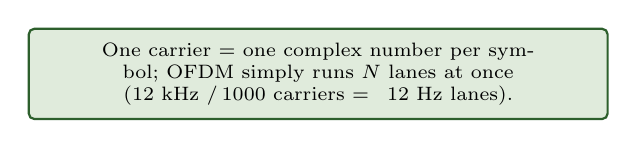
\begin{tikzpicture}
      \node[greencard,text width=7.0cm,font=\scriptsize] {%
        One carrier $=$ one complex number per symbol; OFDM simply runs
        $N$ lanes at once ($12$ kHz $/\,1000$ carriers $=12$ Hz lanes).};
    \end{tikzpicture}
  \end{column}
\end{columns}
\end{frame}

% =====================================================================
% 1b. Each carrier as a clock
% =====================================================================
\begin{frame}{Carriers are clocks}
\stepbadgehdr{1}{each bin will become one rotating clock}
\small
\begin{columns}[T,onlytextwidth]
  \begin{column}{0.40\textwidth}
    \vspace{0.2cm}
    \begin{itemize}\setlength{\itemsep}{0.45em}
      \item Think of \emph{“frequency $\ell$”} as a clock hand whose hand makes $\ell$ full turns in time $T$.
      \item Faster carrier $\to$ faster clock.
      \item The data symbol $d_\ell$ is just where the clock points at $t=0$.
    \end{itemize}

    \vspace{0.20cm}
    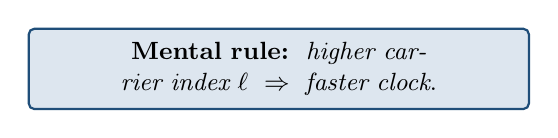
\begin{tikzpicture}
      \node[bluecard,text width=6.0cm] {%
        \textbf{Mental rule:} \,\emph{higher carrier index $\ell$ \;$\Rightarrow$\; faster clock}.
      };
    \end{tikzpicture}
  \end{column}
  \begin{column}{0.58\textwidth}
    \begin{center}
    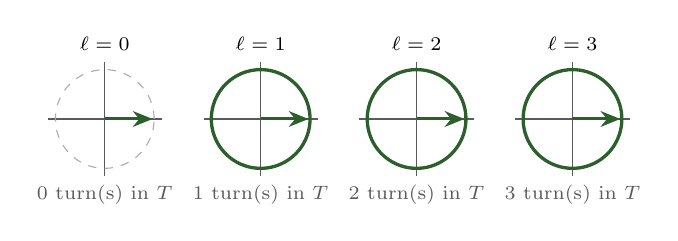
\begin{tikzpicture}[x=0.66cm,y=0.66cm,>=Latex]
      \foreach \k/\dx/\turns in {0/-4.5/0,1/-1.5/1,2/1.5/2,3/4.5/3} {
        \begin{scope}[shift={(\dx,0)}]
          % unit circle + axes
          \draw[inkgray] (-1.1,0) -- (1.1,0);
          \draw[inkgray] (0,-1.1) -- (0,1.1);
          \draw[inkgray!50,dashed] (0,0) circle (0.95);
          % a trail showing how far it has gone at t=T (whole turns)
          \ifnum\k=0
            \draw[accentgreen,line width=1.3pt] (0.95,0) -- (0.95,0);
            \draw[flowarr,color=accentgreen,line width=1.1pt] (0,0) -- (0.92,0);
          \else
            \draw[accentgreen,line width=1.2pt,domain=0:360,samples=80]
              plot ({0.95*cos(\x)},{0.95*sin(\x)});
            \draw[flowarr,color=accentgreen,line width=1.1pt] (0,0) -- (0.92,0);
          \fi
          \node[font=\scriptsize\bfseries] at (0,1.45) {$\ell=\k$};
          \node[font=\scriptsize\color{inkgray}] at (0,-1.45) {\turns\ turn(s) in $T$};
        \end{scope}
      }
    \end{tikzpicture}\\[0.1cm]
    {\scriptsize\itshape\color{inkgray}All clocks start at the same angle and \emph{end at the same angle} (closed loops).}
    \end{center}
  \end{column}
\end{columns}
\end{frame}

% =====================================================================
% 1b2. Where the tone formula comes from, and why it earns the name
% (adapted from doppler_ici_partial_fft_tutorial_grad_version.tex,
%  "Why e^{j2pi l n/N} is a tone")
% =====================================================================
\begin{frame}{Why the clock is the tone $e^{\jj 2\pi \ell n/N}$}
\stepbadgehdr{1}{where the exponential comes from, and why it is called a tone}
\small
\begin{columns}[T,onlytextwidth]
  \begin{column}{0.52\textwidth}
    \vspace{0.05cm}
    \textbf{Where it comes from.}
    Carrier $\ell$ is the clock that makes exactly $\ell$ turns in the
    symbol time $T$: by time $t$ it has swept $\ell\,t/T$ turns, i.e.\ the
    angle $2\pi\ell t/T$. Euler parks a unit arrow at that angle --- this
    is just the continuous carrier $e^{\jj 2\pi f_\ell t}$ with
    $f_\ell=\ell/T$. Sampling $N$ times per symbol, at $t_n=nT/N$:
    \[
      e^{\jj 2\pi \ell t_n/T}
      \;=\;
      e^{\jj 2\pi \ell n/N}
      \qquad\text{($T$ cancels).}
    \]
    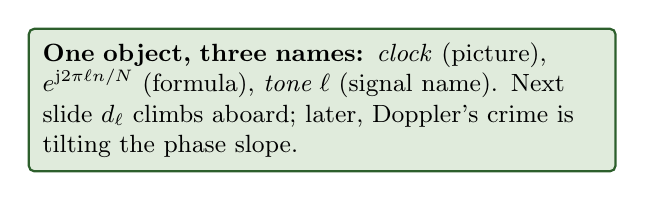
\begin{tikzpicture}
      \node[greencard,text width=7.1cm,align=left] {%
        \textbf{One object, three names:} \emph{clock} (picture),
        $e^{\jj 2\pi \ell n/N}$ (formula), \emph{tone $\ell$} (signal name).
        Next slide $d_\ell$ climbs aboard; later, Doppler's crime is
        tilting the phase slope.};
    \end{tikzpicture}
  \end{column}
  \begin{column}{0.46\textwidth}
    \vspace{0.05cm}
    \textbf{Why ``tone''.}
    A tone is \emph{one} pure frequency, and this arrow cannot hide a
    second one:
    \[
      e^{\jj 2\pi \ell n/N}
      =\cos(2\pi\ell n/N)+\jj\sin(2\pi\ell n/N),
    \]
    a single cosine--sine pair at frequency $f_\ell$, with the \emph{same}
    phase step every sample: $\theta[n{+}1]-\theta[n]=2\pi\ell/N$.
    \begin{center}
    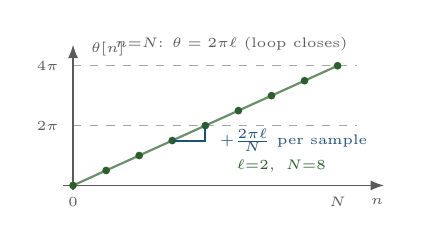
\begin{tikzpicture}[x=0.42cm,y=0.19cm,>=Latex]
      % full-turn gridlines
      \draw[inkgray!55,dashed] (0,4) -- (8.6,4);
      \draw[inkgray!55,dashed] (0,8) -- (8.6,8);
      \node[font=\tiny\color{inkgray},anchor=east] at (-0.15,4) {$2\pi$};
      \node[font=\tiny\color{inkgray},anchor=east] at (-0.15,8) {$4\pi$};
      % axes
      \draw[inkgray,->] (-0.3,0) -- (9.4,0);
      \node[font=\tiny\color{inkgray}] at (9.2,-1.1) {$n$};
      \draw[inkgray,->] (0,-0.3) -- (0,9.4);
      \node[font=\tiny\color{inkgray},anchor=west] at (0.25,9.1) {$\theta[n]$};
      % phase line and samples (l=2, N=8: one quarter turn per sample)
      \draw[accentgreen!70,line width=0.8pt] (0,0) -- (8,8);
      \foreach \n in {0,...,8} {\fill[accentgreen] (\n,\n) circle (1.4pt);}
      % constant step annotation
      \draw[accentblue,line width=0.7pt] (3,3) -- (4,3) -- (4,4);
      \node[font=\tiny\color{accentblue},anchor=west] at (4.15,3.0)
        {$+\tfrac{2\pi\ell}{N}$ per sample};
      % loop closes at n=N
      \node[font=\tiny\color{inkgray},anchor=south east]
        at (8.6,8.35) {$n{=}N$: $\theta=2\pi\ell$ (loop closes)};
      \node[font=\tiny\color{inkgray}] at (0,-1.1) {$0$};
      \node[font=\tiny\color{inkgray}] at (8,-1.1) {$N$};
      \node[font=\tiny\bfseries\color{accentgreen}] at (6.3,1.3) {$\ell{=}2,\ N{=}8$};
    \end{tikzpicture}\\[-0.02cm]
    {\scriptsize\itshape\color{inkgray}phase is a straight line; the slope \emph{is} the frequency}
    \end{center}
  \end{column}
\end{columns}
\end{frame}

% =====================================================================
% 1c. Loading the symbol onto the spinning carrier
% =====================================================================
\begin{frame}{A symbol sets the starting arrow}
\stepbadgehdr{1}{one complex multiplication per sample: lengths multiply, angles add}
\small
\begin{columns}[T,onlytextwidth]
  \begin{column}{0.40\textwidth}
    \vspace{0.10cm}
    ``$d_\ell$ is where the clock points at $t=0$'' is, in math, one
    complex multiplication per sample:
    \[
      s_\ell[n] \;=\; d_\ell \cdot e^{\jj 2\pi \ell n/N}.
    \]
    Write $d_4$ in polar form:
    \[
      d_4 = -1+\jj = \sqrt{2}\, e^{\jj 3\pi/4},
    \]
    so the loaded tone is
    \[
      s_4[n] = \sqrt{2}\, e^{\jj\,(3\pi/4 \,+\, \pi n)} .
    \]
    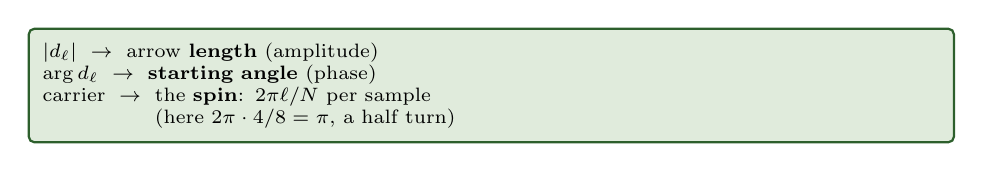
\begin{tikzpicture}
      \node[greencard,text width=0.94\linewidth,align=left,font=\scriptsize] {%
        $|d_\ell|$ $\;\to\;$ arrow \textbf{length} (amplitude)\\
        $\arg d_\ell$ $\;\to\;$ \textbf{starting angle} (phase)\\
        carrier $\;\to\;$ the \textbf{spin}: $2\pi\ell/N$ per sample\\
        \hphantom{carrier $\;\to\;$} (here $2\pi\cdot 4/8=\pi$, a half turn)};
    \end{tikzpicture}
  \end{column}
  \begin{column}{0.58\textwidth}
    \begin{center}
    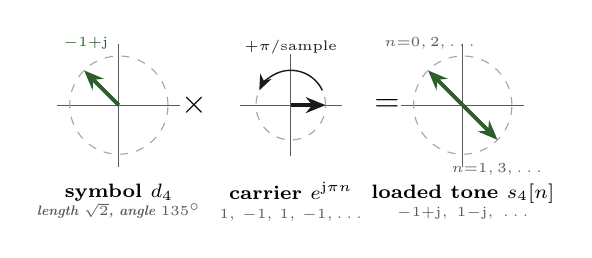
\begin{tikzpicture}[x=0.52cm,y=0.52cm,>=Latex]
      % ---- panel A: the symbol d4 (a static arrow) ----
      \begin{scope}[shift={(-4.2,0)}]
        \draw[inkgray] (-1.50,0) -- (1.50,0);
        \draw[inkgray] (0,-1.50) -- (0,1.50);
        \draw[inkgray!55,dashed] (0,0) circle (1.20);
        \draw[flowarr,color=accentgreen,line width=1.4pt] (0,0) -- (135:1.20);
        \node[font=\tiny\color{accentgreen}] at (118:1.72) {$-1{+}\jj$};
        \node[font=\scriptsize\bfseries,align=center] at (0,-2.35)
          {symbol $d_4$\\[-0.15em]{\tiny\itshape\color{inkgray}length $\sqrt2$, angle $135^\circ$}};
      \end{scope}
      \node[font=\large\bfseries] at (-2.35,0) {$\times$};
      % ---- panel B: the spinning carrier (a unit arrow) ----
      \begin{scope}[shift={(0,0)}]
        \draw[inkgray] (-1.25,0) -- (1.25,0);
        \draw[inkgray] (0,-1.25) -- (0,1.25);
        \draw[inkgray!55,dashed] (0,0) circle (0.85);
        \draw[flowarr,color=ink,line width=1.2pt] (0,0) -- (0:0.85);
        \draw[softarr,color=ink] ({0.85*cos(25)},{0.85*sin(25)}) arc (25:155:0.85);
        \node[font=\tiny\color{ink}] at (90:1.42) {$+\pi$/sample};
        \node[font=\scriptsize\bfseries,align=center] at (0,-2.35)
          {carrier $e^{\jj\pi n}$\\[-0.15em]{\tiny\itshape\color{inkgray}$1,\,-1,\,1,\,-1,\ldots$}};
      \end{scope}
      \node[font=\large\bfseries] at (2.35,0) {$=$};
      % ---- panel C: the loaded tone (symbol arrow, now spinning) ----
      \begin{scope}[shift={(4.2,0)}]
        \draw[inkgray] (-1.50,0) -- (1.50,0);
        \draw[inkgray] (0,-1.50) -- (0,1.50);
        \draw[inkgray!55,dashed] (0,0) circle (1.20);
        \draw[flowarr,color=accentgreen,line width=1.4pt] (0,0) -- (135:1.20);
        \draw[flowarr,color=accentgreen,line width=1.4pt] (0,0) -- (315:1.20);
        \node[font=\tiny\color{inkgray}] at (118:1.72) {$n{=}0,2,\ldots$};
        \node[font=\tiny\color{inkgray}] at (298:1.78) {$n{=}1,3,\ldots$};
        \node[font=\scriptsize\bfseries,align=center] at (0,-2.35)
          {loaded tone $s_4[n]$\\[-0.15em]{\tiny\itshape\color{inkgray}$-1{+}\jj,\ 1{-}\jj,\ \ldots$}};
      \end{scope}
    \end{tikzpicture}
    \end{center}
    \vspace{0.12cm}
    \begin{center}
    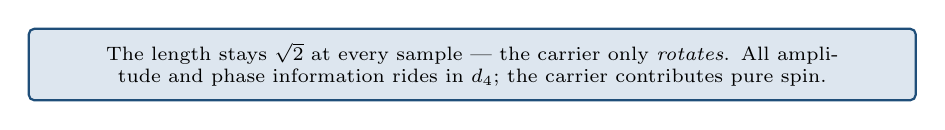
\begin{tikzpicture}
      \node[bluecard,text width=0.90\linewidth,font=\scriptsize] {%
        The length stays $\sqrt 2$ at every sample --- the carrier only \emph{rotates}. All amplitude and phase information rides in $d_4$; the carrier contributes pure spin.};
    \end{tikzpicture}
    \end{center}
  \end{column}
\end{columns}
\bottomnote{This is all ``modulating a carrier'' means here: one complex multiplication per sample. The spinning exponent itself is dissected on the next slide.}
\end{frame}

% =====================================================================
% 1d. Anatomy of a tone (read the exponent inside-out)
% =====================================================================
\begin{frame}{Read the exponent as a turn count}
\stepbadgehdr{1}{read inside-out: it answers ``what fraction of a turn?''}
\small
\begin{columns}[T,onlytextwidth]
  \begin{column}{0.52\textwidth}
    \vspace{0.10cm}
    Read $e^{\jj 2\pi \ell n/N}$ from the inside out:
    \begin{itemize}\setlength{\itemsep}{0.32em}
      \item $n/N$: \emph{how far through the symbol we are} --- sample $n$ out of the $N$ samples in one OFDM symbol.
      \item $\times\,\ell$: carrier $\ell$ goes around $\ell$ times per symbol, so by sample $n$ it has completed $\ell n/N$ \textbf{turns}.
      \item $\times\,2\pi$: convert turns into radians (one full turn $=2\pi$).
      \item $e^{\jj(\cdot)}$: park an \emph{arrow} at that angle on the unit circle; $\jj$ is the $90^\circ$ rotator that makes the arrow two-dimensional instead of a plain cosine.
    \end{itemize}
    \vspace{0.05cm}
    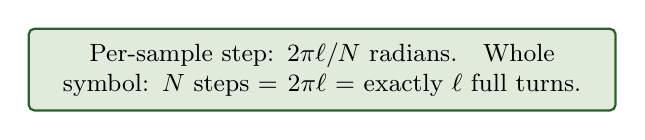
\begin{tikzpicture}
      \node[greencard,text width=7.1cm] {%
        Per-sample step: $2\pi\ell/N$ radians.\quad
        Whole symbol: $N$ steps $=2\pi\ell$ $=$ exactly $\ell$ full turns.};
    \end{tikzpicture}
  \end{column}
  \begin{column}{0.46\textwidth}
    \begin{center}
    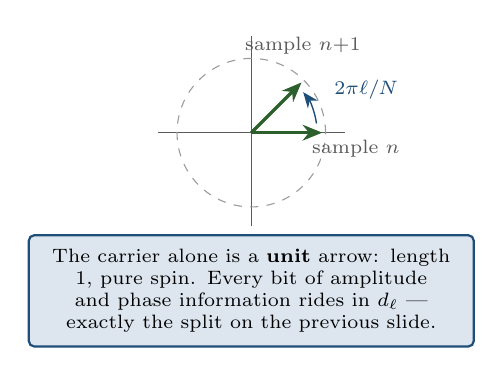
\begin{tikzpicture}[x=0.82cm,y=0.82cm,>=Latex]
      \draw[inkgray] (-1.45,0.55) -- (1.45,0.55);
      \draw[inkgray] (0,-0.90) -- (0,2.05);
      \draw[inkgray!60,dashed] (0,0.55) circle (1.15);
      \draw[flowarr,color=accentgreen,line width=1.2pt] (0,0.55) -- (1.10,0.55);
      \draw[flowarr,color=accentgreen,line width=1.2pt] (0,0.55)
        -- ({1.10*cos(45)},{0.55+1.10*sin(45)});
      \draw[softarr,color=accentblue]
        ({1.02*cos(8)},{0.55+1.02*sin(8)}) arc (8:38:1.02);
      \node[font=\scriptsize\color{accentblue}] at (1.78,1.22) {$2\pi\ell/N$};
      \node[font=\scriptsize\color{inkgray}] at (1.62,0.30) {sample $n$};
      \node[font=\scriptsize\color{inkgray}] at (0.80,1.90) {sample $n{+}1$};
      \node[bluecard,text width=5.3cm,font=\scriptsize] at (0,-1.90) {%
        The carrier alone is a \textbf{unit} arrow: length $1$, pure spin.
        Every bit of amplitude and phase information rides in $d_\ell$ ---
        exactly the split on the previous slide.};
    \end{tikzpicture}
    \end{center}
  \end{column}
\end{columns}
\bottomnote{Same object in continuous time: $e^{\jj 2\pi f_\ell t}$ with $f_\ell=\ell/T$; sampling at $t=nT/N$ gives the discrete formula above.}
\end{frame}

% =====================================================================
% 1e. Worked example: l=2, N=8 (a quarter turn per sample)
% =====================================================================
\begin{frame}{A quarter-turn tone you can check}
\stepbadgehdr{1}{one concrete tone you can compute in your head}
\small
\begin{columns}[T,onlytextwidth]
  \begin{column}{0.50\textwidth}
    \vspace{0.10cm}
    Per-sample step for this tone:
    \[
      \frac{2\pi\ell}{N}
      =\frac{2\pi\cdot 2}{8}
      =\frac{\pi}{2}
      \qquad\text{(a quarter turn).}
    \]
    So the samples simply walk the quadrant points:
    \[
      e^{\jj\pi n/2}
      = 1,\ \jj,\ -1,\ -\jj,\ 1,\ \jj,\ -1,\ -\jj .
    \]
    \vspace{0.05cm}
    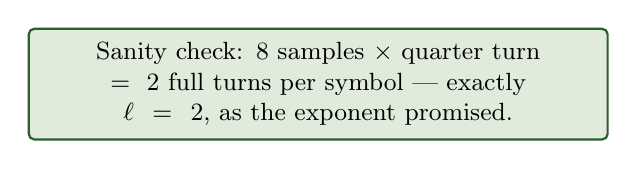
\begin{tikzpicture}
      \node[greencard,text width=7.0cm] {%
        Sanity check: $8$ samples $\times$ quarter turn $=2$ full turns
        per symbol --- exactly $\ell=2$, as the exponent promised.};
    \end{tikzpicture}
  \end{column}
  \begin{column}{0.48\textwidth}
    \begin{center}
    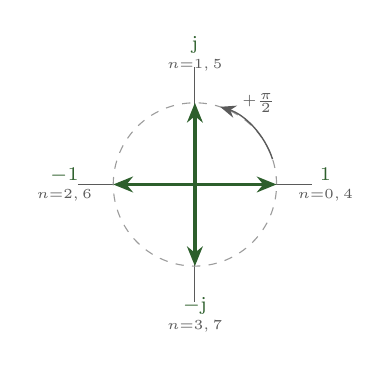
\begin{tikzpicture}[x=0.85cm,y=0.85cm,>=Latex]
      \draw[inkgray] (-1.75,0) -- (1.75,0);
      \draw[inkgray] (0,-1.75) -- (0,1.75);
      \draw[inkgray!60,dashed] (0,0) circle (1.22);
      \foreach \ang/\lab/\ns in {%
        0/{$1$}/{$n{=}0,4$},
        90/{$\jj$}/{$n{=}1,5$},
        180/{$-1$}/{$n{=}2,6$},
        270/{$-\jj$}/{$n{=}3,7$}}{
        \draw[flowarr,color=accentgreen,line width=1.3pt] (0,0) -- (\ang:1.22);
        \node[font=\scriptsize\bfseries\color{accentgreen},align=center]
          at (\ang:1.95) {\lab\\[-0.15em]{\tiny\color{inkgray}\ns}};
      }
      \draw[softarr,color=inkgray] ({1.22*cos(18)},{1.22*sin(18)}) arc (18:72:1.22);
      \node[font=\tiny\color{inkgray}] at (52:1.55) {$+\frac{\pi}{2}$};
    \end{tikzpicture}
    \end{center}
    \vspace{-0.05cm}
    \begin{center}
      {\scriptsize\itshape\color{inkgray}
      Each arrow position is visited twice: the clock laps the circle two times.}
    \end{center}
  \end{column}
\end{columns}
\bottomnote{Tone $4$ plays the same game with a half-turn step: $e^{\jj\pi n}=1,-1,1,-1,\ldots$ --- you will meet it on the IFFT slide.}
\end{frame}

% =====================================================================
% 1f. IFFT builds the transmit waveform
% =====================================================================
\begin{frame}{The IFFT adds the clocks}
\stepbadgehdr{1}{transmission is the sum of all spinning tones}
\small
\begin{columns}[T,onlytextwidth]
  \begin{column}{0.50\textwidth}
    The transmitter takes the tone vector $\mathbf d$ and performs an IFFT:
    \[
      x[n]
      =\frac{1}{8}\sum_{\ell=0}^{7}
        d_\ell e^{\jj2\pi \ell n/8},
      \qquad n=0,\ldots,7.
    \]
    So tone $\ell$ contributes a small rotating sequence:
    \[
      d_\ell e^{\jj2\pi \ell n/8}.
    \]
    In a clean channel, the receiver sees the same samples:
    \[
      r[n]=x[n].
    \]
  \end{column}
  \begin{column}{0.48\textwidth}
    \begin{center}
    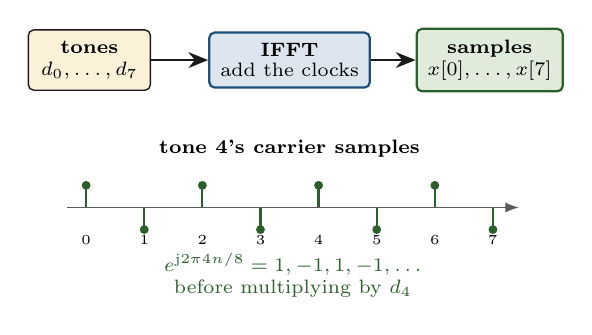
\begin{tikzpicture}[x=0.82cm,y=0.78cm,>=Latex]
      % top row: tones -> IFFT -> samples, with generous gaps
      \node[notecard,minimum width=1.55cm,inner sep=4pt,
            font=\scriptsize,align=center] (tones)
        at (-3.10,1.05) {\textbf{tones}\\$d_0,\ldots,d_7$};
      \node[bluecard,minimum width=1.50cm,inner sep=4pt,
            font=\scriptsize\bfseries,align=center] (ifft) at (0.00,1.05)
        {IFFT\\[-0.1em]\scriptsize\mdseries add the clocks};
      \node[greencard,minimum width=1.85cm,inner sep=4pt,
            font=\scriptsize,align=center] (samples)
        at (3.10,1.05) {\textbf{samples}\\$x[0],\ldots,x[7]$};
      \draw[flowarr,color=ink,line width=0.8pt] (tones.east) -- (ifft.west);
      \draw[flowarr,color=ink,line width=0.8pt] (ifft.east) -- (samples.west);

      % bottom: tone 4 samples stem-plot
      \node[font=\scriptsize\bfseries] at (0,-0.40) {tone 4's carrier samples};
      \foreach \n in {0,...,7} {
        \pgfmathsetmacro{\xx}{-3.15+0.9*\n}
        \pgfmathsetmacro{\yy}{-1.35+0.36*cos(180*\n)}
        \draw[accentgreen,line width=0.8pt] (\xx,-1.35) -- (\xx,\yy);
        \fill[accentgreen] (\xx,\yy) circle (1.6pt);
        \node[font=\tiny] at (\xx,-1.88) {\n};
      }
      \draw[inkgray,->] (-3.45,-1.35) -- (3.55,-1.35);
      \node[font=\scriptsize\color{accentgreen},align=center] at (0.05,-2.45)
        {$e^{\jj2\pi 4 n/8}=1,-1,1,-1,\ldots$\\before multiplying by $d_4$};
    \end{tikzpicture}
    \end{center}
  \end{column}
\end{columns}
\bottomnote{The IFFT builds the transmitted waveform by adding all carriers together.}
\end{frame}

% =====================================================================
% 1g. Why orthogonality works (clocks and closed loops)
% =====================================================================
\begin{frame}{Closed loops let the FFT separate carriers}
\stepbadgehdr{1}{clean OFDM = every wrong clock closes a loop}
\small
\begin{columns}[T,onlytextwidth]
  \begin{column}{0.48\textwidth}
    \vspace{0.15cm}
    \begin{itemize}\setlength{\itemsep}{0.40em}
      \item FFT bin $k$ \emph{listens} by multiplying with a clock spinning \textbf{backward} at rate $k$.
      \item Carrier $\ell$, after that, has rate $\ell-k$ (\emph{leftover spin}).
      \item Average over one symbol $\rightarrow$ closed loops cancel to zero. Only $\ell=k$ survives.
    \end{itemize}
    \[
      c_{k,\ell}^{(0)}
      = \int_0^1 e^{\jj 2\pi(\ell-k)t}\,dt
      =
      \begin{cases}
        1, & \ell = k,\\[0.1em]
        0, & \ell \ne k.
      \end{cases}
    \]
    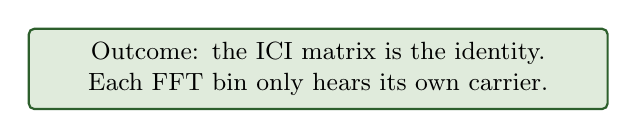
\begin{tikzpicture}
      \node[greencard,text width=7.0cm] {%
        Outcome: the ICI matrix is the identity. Each FFT bin only hears its own carrier.
      };
    \end{tikzpicture}
  \end{column}
  \begin{column}{0.50\textwidth}
    \begin{center}
    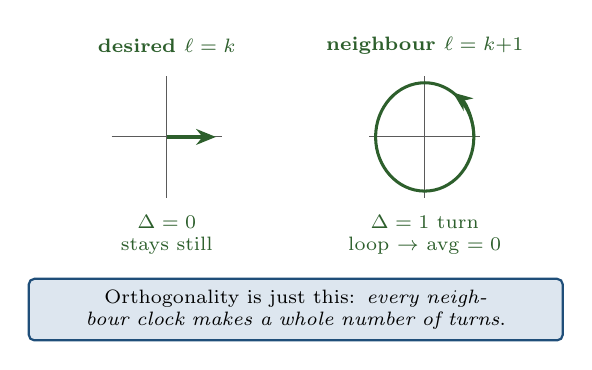
\begin{tikzpicture}[x=0.78cm,y=0.86cm,>=Latex]
      % desired carrier (compact)
      \node[font=\scriptsize\bfseries\color{accentgreen}] at (-2.1,2.05) {desired $\ell=k$};
      \draw[inkgray] (-3.0,0.7) -- (-1.2,0.7);
      \draw[inkgray] (-2.1,-0.20) -- (-2.1,1.60);
      \draw[flowarr,color=accentgreen,line width=1.2pt] (-2.1,0.7) -- (-1.30,0.7);
      \node[font=\scriptsize\color{accentgreen},align=center] at (-2.1,-0.75)
        {$\Delta=0$\\stays still};

      % neighbour, integer turn (compact)
      \node[font=\scriptsize\bfseries\color{accentgreen}] at (2.1,2.05) {neighbour $\ell=k{+}1$};
      \draw[inkgray] (1.2,0.7) -- (3.0,0.7);
      \draw[inkgray] (2.1,-0.20) -- (2.1,1.60);
      \draw[accentgreen,line width=1.1pt] (2.1,0.7) circle (0.80);
      \draw[flowarr,color=accentgreen,line width=1.0pt] (2.90,0.7) arc (0:55:0.80);
      \node[font=\scriptsize\color{accentgreen},align=center] at (2.1,-0.75)
        {$\Delta=1$ turn\\loop $\to$ avg $=0$};

      % bottom callout (narrower)
      \node[bluecard,text width=6.5cm,inner sep=4pt,font=\scriptsize] at (0,-1.85) {%
        Orthogonality is just this: \emph{every neighbour clock makes a whole number of turns}.
      };
    \end{tikzpicture}
    \end{center}
  \end{column}
\end{columns}
\end{frame}
% =====================================================================
% 1h. De-spin: bin l freezes tone l (the remaining phasor stands still)
% =====================================================================
\begin{frame}{De-spinning freezes the wanted tone}
\stepbadgehdr{1}{multiply by the backward clock; the remaining phasor stands still}
\small
\begin{columns}[T,onlytextwidth]
  \begin{column}{0.52\textwidth}
    Bin $\ell$ owns the \emph{backward} clock $e^{-\jj 2\pi \ell n/N}$.
    Apply it to our $\ell=2$, $N=8$ tone, sample by sample:
    \[
      \begin{array}{c|ccccc}
        n & 0 & 1 & 2 & 3 & \cdots\\ \hline
        \text{tone } e^{\jj\pi n/2} & 1 & \jj & -1 & -\jj & \cdots\\
        \text{clock } e^{-\jj\pi n/2} & 1 & -\jj & -1 & \jj & \cdots\\ \hline
        \text{product} & 1 & 1 & 1 & 1 & \cdots
      \end{array}
    \]
    Every sample lands on the \emph{same} point: the remaining phasor
    does not spin at all. It \textbf{stands still} at $d_2$, and
    averaging $N$ identical arrows returns $d_2$ exactly.
  \end{column}
  \begin{column}{0.46\textwidth}
    \begin{center}
    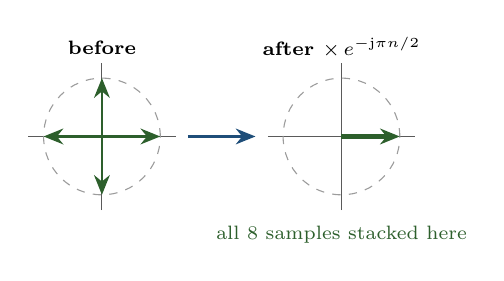
\begin{tikzpicture}[x=0.78cm,y=0.78cm,>=Latex]
      \node[font=\scriptsize\bfseries] at (-1.95,2.00) {before};
      \draw[inkgray] (-3.15,0.55) -- (-0.75,0.55);
      \draw[inkgray] (-1.95,-0.65) -- (-1.95,1.75);
      \draw[inkgray!60,dashed] (-1.95,0.55) circle (0.95);
      \foreach \ang in {0,90,180,270} {
        \draw[flowarr,color=accentgreen,line width=1.0pt] (-1.95,0.55) -- ++(\ang:0.95);
      }
      \node[font=\scriptsize\bfseries] at (1.95,2.00) {after $\times\, e^{-\jj\pi n/2}$};
      \draw[inkgray] (0.75,0.55) -- (3.15,0.55);
      \draw[inkgray] (1.95,-0.65) -- (1.95,1.75);
      \draw[inkgray!60,dashed] (1.95,0.55) circle (0.95);
      \draw[flowarr,color=accentgreen,line width=2.0pt] (1.95,0.55) -- ++(0:0.95);
      \node[font=\scriptsize\color{accentgreen}] at (1.95,-1.05) {all $8$ samples stacked here};
      \draw[flowarr,color=accentblue,line width=0.9pt] (-0.55,0.55) -- (0.55,0.55);
    \end{tikzpicture}
    \end{center}
    \vspace{0.12cm}
    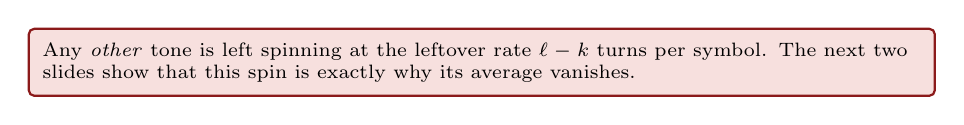
\begin{tikzpicture}
      \node[redcard,text width=0.92\linewidth,font=\scriptsize,align=left] {%
        Any \emph{other} tone is left spinning at the leftover rate
        $\ell-k$ turns per symbol. The next two slides show that this
        spin is exactly why its average vanishes.};
    \end{tikzpicture}
  \end{column}
\end{columns}
\bottomnote{``De-spin'' is one row of the FFT: multiply by $e^{-\jj 2\pi k n/N}$, then average. Decoding $=$ freeze your own tone, let every other tone keep spinning.}
\end{frame}

% =====================================================================
% 1i. FFT bin 4 decodes
% =====================================================================
\begin{frame}{Bin 4 asks for the fourth clock}
\stepbadgehdr{1}{one FFT row is a matched clock plus an average}
\small
\begin{columns}[T,onlytextwidth]
  \begin{column}{0.50\textwidth}
    Receiver bin $4$ multiplies by the opposite fourth carrier and averages:
    \[
      y_4
      =\sum_{n=0}^{7} r[n]e^{-\jj2\pi4n/8}.
    \]
    Substitute the transmitted sum:
    \[
      y_4
      =\sum_{\ell=0}^{7}d_\ell
        \underbrace{\frac{1}{8}\sum_{n=0}^{7}
        e^{\jj2\pi(\ell-4)n/8}}_{\text{how much tone }\ell\text{ enters bin }4}.
    \]
    This bracket is the clean OFDM coupling coefficient $c_{4,\ell}^{(0)}$.
  \end{column}
  \begin{column}{0.48\textwidth}
    \begin{center}
    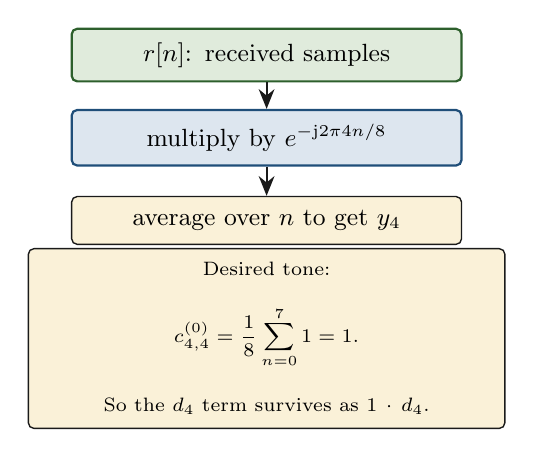
\begin{tikzpicture}[x=1cm,y=1cm,>=Latex]
      \node[greencard,text width=4.6cm] (r) at (0,1.40) {$r[n]$: received samples};
      \node[bluecard,text width=4.6cm] (mix) at (0,0.35) {multiply by $e^{-\jj2\pi4n/8}$};
      \node[notecard,text width=4.6cm] (avg) at (0,-0.70) {average over $n$ to get $y_4$};
      \draw[flowarr,color=ink] (r) -- (mix);
      \draw[flowarr,color=ink] (mix) -- (avg);

      \node[notecard,text width=5.7cm,font=\scriptsize] at (0,-2.20) {%
        Desired tone:
        \[
          c_{4,4}^{(0)}=\frac{1}{8}\sum_{n=0}^{7}1=1.
        \]
        So the $d_4$ term survives as $1\cdot d_4$.};
    \end{tikzpicture}
    \end{center}
  \end{column}
\end{columns}
\bottomnote{FFT bin 4 is one row of the FFT matrix: a matched filter for carrier 4.}
\end{frame}
% =====================================================================
% 1j. Clean numerical example
% =====================================================================
\begin{frame}{A neighbor disappears when its loop closes}
\stepbadgehdr{1}{this is the zero Doppler will later break}
\small
\begin{columns}[T,onlytextwidth]
  \begin{column}{0.50\textwidth}
    For the neighbour tone $\ell=5$, bin $4$ sees one leftover turn:
    \[
      c_{4,5}^{(0)}
      =\frac{1}{8}\sum_{n=0}^{7}e^{\jj2\pi(5-4)n/8}
      =\frac{1}{8}\sum_{n=0}^{7}e^{\jj2\pi n/8}.
    \]
    The eight arrows are equally spaced around the unit circle, so their sum is zero:
    \[
      c_{4,5}^{(0)}=0,
      \qquad
      d_5\text{ contributes }c_{4,5}^{(0)}d_5=0.
    \]
    Continuous version:
    \(\int_0^1 e^{\jj2\pi(5-4)t}\,dt=0\).
  \end{column}
  \begin{column}{0.48\textwidth}
    \begin{center}
    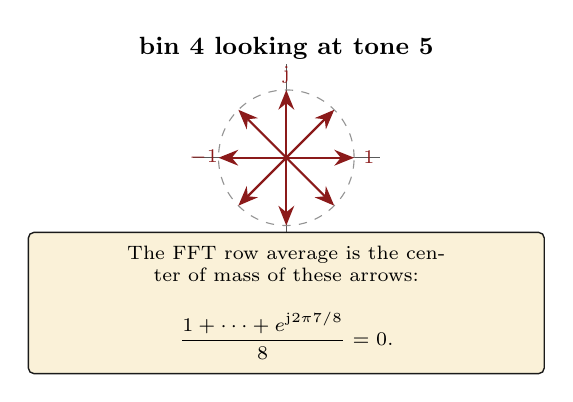
\begin{tikzpicture}[x=0.82cm,y=0.82cm,>=Latex]
      \node[font=\small\bfseries] at (0,2.10) {bin 4 looking at tone 5};
      \draw[inkgray] (-1.45,0.40) -- (1.45,0.40);
      \draw[inkgray] (0,-1.05) -- (0,1.85);
      \draw[inkgray!65,dashed] (0,0.40) circle (1.05);
      \foreach \ang in {0,45,...,315} {
        \draw[flowarr,color=accentred,line width=0.8pt] (0,0.40) -- ++(\ang:1.05);
      }
      \foreach \ang/\lab in {0/$1$,90/$\jj$,180/$-1$,270/$-\jj$} {
        \node[font=\scriptsize\color{accentred}] at ({1.28*cos(\ang)},{0.40+1.28*sin(\ang)}) {\lab};
      }
      \node[notecard,text width=6.2cm,font=\scriptsize] at (0,-1.85) {%
        The FFT row average is the center of mass of these arrows:
        \[
          \frac{1+\cdots+e^{\jj2\pi7/8}}{8}=0.
        \]};
    \end{tikzpicture}
    \end{center}
  \end{column}
\end{columns}
\bottomnote{Doppler breaks this benchmark by making the leftover turn count non-integer.}
\end{frame}
% =====================================================================
% 1k. Common phase is a useful non-example
% =====================================================================
\begin{frame}{Common phase rotates everything together}
\stepbadgehdr{1}{first rule out the harmless kind of rotation}
\small
\begin{columns}[T,onlytextwidth]
  \begin{column}{0.48\textwidth}
    A constant phase shift rotates the \emph{whole} OFDM symbol by the same angle:
    \[
      r(t)=e^{\jj\phi}\sum_\ell d_\ell e^{\jj2\pi f_\ell t}.
    \]
    Bin $k$ still sees
    \[
      y_k=e^{\jj\phi}
      \sum_\ell d_\ell
      \int_0^T e^{\jj2\pi(f_\ell-f_k)t}\,dt
      =e^{\jj\phi}d_k .
    \]
    The constellation rotates, but the off-diagonal carrier terms still integrate to zero.
    To create ICI, the channel must change \emph{relative} clock rates.
  \end{column}
  \begin{column}{0.50\textwidth}
    \begin{center}
    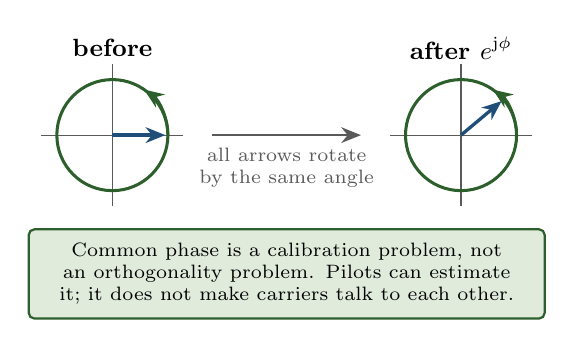
\begin{tikzpicture}[x=0.82cm,y=0.82cm,>=Latex]
      \node[font=\small\bfseries] at (-2.7,2.05) {before};
      \draw[inkgray] (-3.8,0.7) -- (-1.6,0.7);
      \draw[inkgray] (-2.7,-0.4) -- (-2.7,1.8);
      \draw[accentgreen,line width=1.1pt] (-2.7,0.7) circle (0.86);
      \draw[flowarr,color=accentgreen,line width=1.0pt] (-1.84,0.7) arc (0:55:0.86);
      \draw[flowarr,color=accentblue,line width=1.2pt] (-2.7,0.7) -- ++(0.82,0.0);

      \node[font=\small\bfseries] at (2.7,2.05) {after $e^{\jj\phi}$};
      \draw[inkgray] (1.6,0.7) -- (3.8,0.7);
      \draw[inkgray] (2.7,-0.4) -- (2.7,1.8);
      \draw[accentgreen,line width=1.1pt] (2.7,0.7) circle (0.86);
      \draw[flowarr,color=accentgreen,line width=1.0pt] (3.56,0.7) arc (0:55:0.86);
      \draw[flowarr,color=accentblue,line width=1.2pt] (2.7,0.7) -- ++(40:0.82);

      \draw[flowarr,color=inkgray,line width=0.8pt] (-1.15,0.70) -- (1.15,0.70);
      \node[font=\scriptsize\color{inkgray},align=center] at (0,0.20)
        {all arrows rotate\\by the same angle};
      \node[greencard,text width=6.2cm,font=\scriptsize] at (0,-1.45) {%
        Common phase is a calibration problem, not an orthogonality problem. Pilots can estimate it; it does not make carriers talk to each other.};
    \end{tikzpicture}
    \end{center}
  \end{column}
\end{columns}
\end{frame}
% =====================================================================
% 2a. How Doppler is created (math but with intuition first)
% =====================================================================
\begin{frame}{Doppler changes the clock rates}
\stepbadgehdr{2}{wideband motion changes relative spin rates, not just phase}
\small
\begin{columns}[T,onlytextwidth]
  \begin{column}{0.48\textwidth}
    \vspace{0.15cm}
    \textbf{Plain version.}
    Relative motion makes the path length grow or shrink \emph{during} the symbol. The whole waveform gets \emph{time-scaled} by a factor $1+a$:
    \[
      x(t-\tau(t))
      \;=\;
      x\!\big((1+a)\,t - \tau_0\big),
      \quad a=\frac{v}{c_{\mathrm w}} .
    \]
    \textbf{Effect on each carrier.}
    The frequency a receiver sees is
    \[
      f_\ell^{\rx} \;=\; (1+a)\,f_\ell \;+\; \nu,
    \]
    where $\nu$ is any additional common (narrow-band) offset.
    \vspace{0.05cm}
    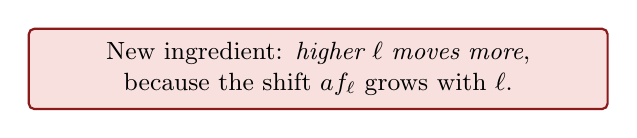
\begin{tikzpicture}
      \node[redcard,text width=7.0cm] {%
        New ingredient: \emph{higher $\ell$ moves more}, because the shift $a f_\ell$ grows with $\ell$.
      };
    \end{tikzpicture}
  \end{column}
  \begin{column}{0.50\textwidth}
    \begin{center}
    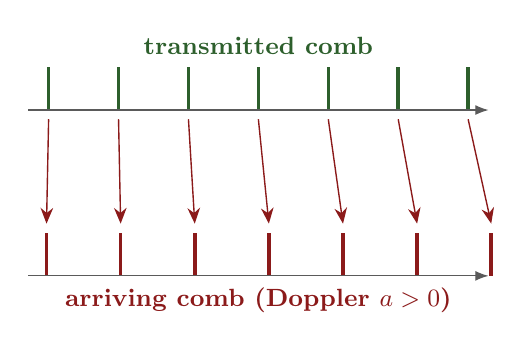
\begin{tikzpicture}[x=0.74cm,y=0.78cm,>=Latex]
      % clean comb on top
      \node[font=\small\bfseries\color{accentgreen}] at (0,2.05) {transmitted comb};
      \foreach \x in {-3.6,-2.4,-1.2,0,1.2,2.4,3.6} {
        \draw[accentgreen,line width=1.3pt] (\x,1.0) -- (\x,1.7);
      }
      \draw[inkgray,->] (-3.95,1.0) -- (3.95,1.0);

      % connecting "Doppler scaling" arrows between the two combs (away from any label)
      \foreach \x in {-3.6,-2.4,-1.2,0,1.2,2.4,3.6} {
        \pgfmathsetmacro{\xs}{\x*1.06+0.18}
        \draw[softarr,color=accentred] (\x,0.85) -- (\xs,-0.85);
      }

      % scaled comb on bottom (label moved BELOW the comb, out of the arrows)
      \foreach \x in {-3.6,-2.4,-1.2,0,1.2,2.4,3.6} {
        \pgfmathsetmacro{\xs}{\x*1.06+0.18}
        \draw[accentred,line width=1.3pt] (\xs,-1.7) -- (\xs,-1.0);
      }
      \draw[inkgray,->] (-3.95,-1.7) -- (3.95,-1.7);
      \node[font=\small\bfseries\color{accentred}] at (0,-2.10) {arriving comb (Doppler $a>0$)};
    \end{tikzpicture}
    \end{center}
    \vspace{-0.10cm}
    \begin{center}
      \scriptsize\itshape\color{inkgray}
      Every comb tooth moves; outer teeth move more than inner ones.
    \end{center}
  \end{column}
\end{columns}
\end{frame}
% =====================================================================
% 2b. Why Delta f times t is a turn count
% =====================================================================
\begin{frame}{Turn count is frequency difference times time}
\stepbadgehdr{2}{frequency difference $\times$ time = relative turns}
\small
\begin{columns}[T,onlytextwidth]
  \begin{column}{0.46\textwidth}
    Once carrier $\ell$ is viewed from bin $k$, the relative rate is
    \[
      \Delta f=f_\ell^{\rx}-f_k.
    \]
    Frequency is cycles per second. Therefore
    \[
      \underbrace{\Delta f}_{\text{cycles/sec}}
      \times
      \underbrace{t}_{\text{sec}}
      =
      \underbrace{\Delta f\,t}_{\text{cycles}}.
    \]
    The complex exponential turns cycles into angle:
    \[
      e^{\jj2\pi\Delta f t}
      \quad\text{has phase}\quad
      2\pi\Delta f t.
    \]
  \end{column}
  \begin{column}{0.52\textwidth}
    \begin{center}
    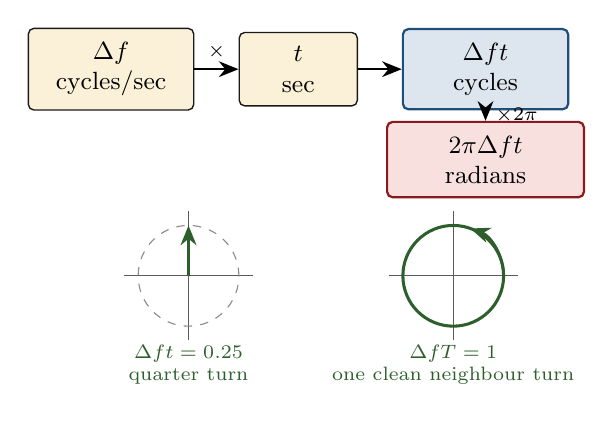
\begin{tikzpicture}[x=0.82cm,y=0.82cm,>=Latex]
      \node[notecard,minimum width=2.1cm] (rate) at (-3.2,1.45) {$\Delta f$\\cycles/sec};
      \node[notecard,minimum width=1.5cm] (time) at (-0.3,1.45) {$t$\\sec};
      \node[bluecard,minimum width=2.1cm] (turns) at (2.6,1.45) {$\Delta f t$\\cycles};
      \node[redcard,minimum width=2.5cm] (phase) at (2.6,0.05) {$2\pi\Delta f t$\\radians};
      \draw[flowarr] (rate) -- node[above,font=\scriptsize] {$\times$} (time);
      \draw[flowarr] (time) -- (turns);
      \draw[flowarr] (turns) -- node[right,font=\scriptsize] {$\times 2\pi$} (phase);

      \begin{scope}[shift={(-2.0,-1.75)}]
        \draw[inkgray] (-1.0,0) -- (1.0,0);
        \draw[inkgray] (0,-1.0) -- (0,1.0);
        \draw[inkgray!70,dashed] (0,0) circle (0.78);
        \draw[flowarr,color=accentgreen,line width=1.2pt] (0,0) -- (0,0.78);
        \node[font=\scriptsize\color{accentgreen},align=center] at (0,-1.38)
          {$\Delta f t=0.25$\\quarter turn};
      \end{scope}
      \begin{scope}[shift={(2.1,-1.75)}]
        \draw[inkgray] (-1.0,0) -- (1.0,0);
        \draw[inkgray] (0,-1.0) -- (0,1.0);
        \draw[accentgreen,line width=1.1pt] (0,0) circle (0.78);
        \draw[flowarr,color=accentgreen,line width=1.0pt] (0.78,0) arc (0:70:0.78);
        \node[font=\scriptsize\color{accentgreen},align=center] at (0,-1.38)
          {$\Delta fT=1$\\one clean neighbour turn};
      \end{scope}
    \end{tikzpicture}
    \end{center}
  \end{column}
\end{columns}
\bottomnote{OFDM spacing is chosen so a clean neighbour has $\Delta fT=1$ full turn. Doppler changes it to $1+\epsilon$, so the loop misses closure.}
\end{frame}
% =====================================================================
% 3a. ICI as an unfinished loop
% =====================================================================
\begin{frame}{ICI begins when the loop misses closure}
\stepbadgehdr{3}{the failed cancellation loop becomes a leakage coefficient}
\small
\begin{columns}[T,onlytextwidth]
  \begin{column}{0.48\textwidth}
    \textbf{No Doppler.}
    Leftover spin between carrier $\ell$ and bin $k$:
    \[
      \Delta_{k,\ell}=\ell-k.
    \]
    Every neighbour gets a whole number of turns, so
    \[
      c_{k,\ell}=\int_0^1 e^{\jj 2\pi \Delta_{k,\ell}t}\,dt = 0,\quad \ell\ne k.
    \]

    \begin{center}
    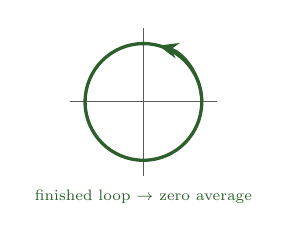
\begin{tikzpicture}[scale=0.78,transform shape]
      \draw[inkgray] (-1.2,0) -- (1.2,0);
      \draw[inkgray] (0,-1.2) -- (0,1.2);
      \draw[accentgreen,line width=1.2pt] (0,0) circle (0.95);
      \draw[flowarr,color=accentgreen,line width=1.0pt] (0.95,0) arc (0:75:0.95);
      \node[font=\scriptsize\color{accentgreen}] at (0,-1.55)
        {finished loop $\to$ zero average};
    \end{tikzpicture}
    \end{center}
  \end{column}
  \begin{column}{0.48\textwidth}
    \textbf{With residual Doppler.}
    Each $\ell$ becomes
    \[
      f_\ell^{\rx}=(1+a)\ell+\nu,\quad
      \Delta_{k,\ell}=(\ell-k)+\nu+a\ell.
    \]
    For neighbour $\ell=k+1$:
    \[
      \Delta_{k,k+1}=1+\nu+a(k+1)
      \;\Rightarrow\; c_{k,k+1}\ne 0.
    \]

    \begin{center}
    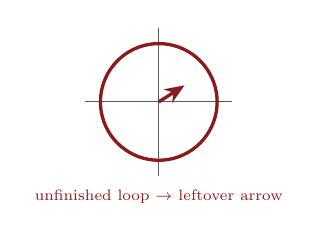
\begin{tikzpicture}[scale=0.78,transform shape]
      \draw[inkgray] (-1.2,0) -- (1.2,0);
      \draw[inkgray] (0,-1.2) -- (0,1.2);
      \draw[accentred,line width=1.2pt,domain=0:445,samples=90]
        plot ({0.95*cos(\x)},{0.95*sin(\x)});
      \draw[flowarr,color=accentred,line width=1.2pt] (0,0) -- (0.42,0.27);
      \node[font=\scriptsize\color{accentred}] at (0,-1.55)
        {unfinished loop $\to$ leftover arrow};
    \end{tikzpicture}
    \end{center}
  \end{column}
\end{columns}
\end{frame}

% =====================================================================
% 3b. Frequency domain (sinc grid)
% =====================================================================
\begin{frame}{The same leak shows up as sinc tails}
\stepbadgehdr{3}{same coefficient, different picture}
\small
\begin{columns}[T,onlytextwidth]
  \begin{column}{0.49\textwidth}
    \textbf{Clean OFDM.}\,\, Each carrier is a $\sinc$ centred on its frequency. The FFT samples the spectrum at the bin grid — and lands \emph{on every other carrier's zero}.
    \begin{center}
    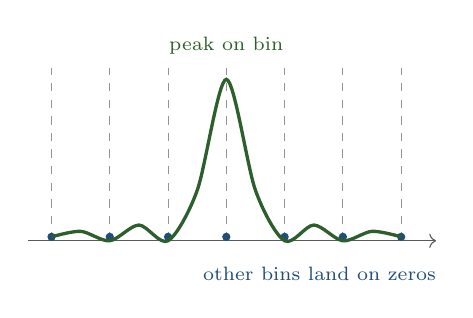
\begin{tikzpicture}[x=0.74cm,y=1.0cm]
      \draw[inkgray,->] (-3.4,0) -- (3.6,0);
      \foreach \k in {-3,-2,-1,0,1,2,3} {
        \draw[inkgray!65,dashed] (\k,0) -- (\k,2.2);
        \fill[accentblue] (\k,0.05) circle (1.5pt);
      }
      \draw[accentgreen,line width=1.2pt,smooth]
        plot coordinates {(-3,0.05)(-2.5,0.12)(-2,0.0)(-1.5,0.20)(-1,0)(-0.5,0.64)(0,2.05)(0.5,0.64)(1,0)(1.5,0.20)(2,0)(2.5,0.12)(3,0.05)};
      \node[font=\scriptsize\color{accentgreen}] at (0,2.48) {peak on bin};
      \node[font=\scriptsize\color{accentblue}] at (1.6,-0.42) {other bins land on zeros};
    \end{tikzpicture}
    \end{center}
  \end{column}
  \begin{column}{0.49\textwidth}
    \textbf{With Doppler.}\,\, The whole carrier sits a fraction of a bin off-grid. The FFT now samples \emph{the tails}, and that is exactly the ICI.
    \begin{center}
    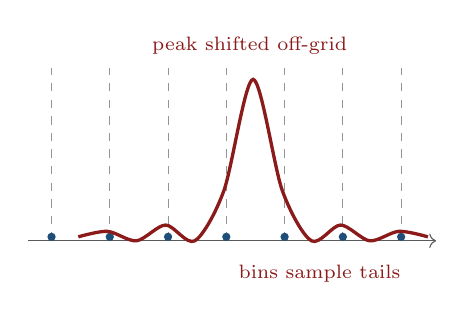
\begin{tikzpicture}[x=0.74cm,y=1.0cm]
      \draw[inkgray,->] (-3.4,0) -- (3.6,0);
      \foreach \k in {-3,-2,-1,0,1,2,3} {
        \draw[inkgray!65,dashed] (\k,0) -- (\k,2.2);
        \fill[accentblue] (\k,0.05) circle (1.5pt);
      }
      \begin{scope}[xshift=0.34cm]
      \draw[accentred,line width=1.2pt,smooth]
        plot coordinates {(-3,0.05)(-2.5,0.12)(-2,0.0)(-1.5,0.20)(-1,0)(-0.5,0.64)(0,2.05)(0.5,0.64)(1,0)(1.5,0.20)(2,0)(2.5,0.12)(3,0.05)};
      \end{scope}
      \node[font=\scriptsize\color{accentred}] at (0.4,2.48) {peak shifted off-grid};
      \node[font=\scriptsize\color{accentred}] at (1.6,-0.42) {bins sample tails};
    \end{tikzpicture}
    \end{center}
  \end{column}
\end{columns}
\bottomnote{The time-domain residual phasor and the frequency-domain sinc tail are the same ICI coefficient seen two ways.}
\end{frame}

% =====================================================================
% 3c. A small numerical example
% =====================================================================
\begin{frame}{One leak you can verify by hand}
\stepbadgehdr{3}{plug the workbench numbers in}
\small
\begin{columns}[T,onlytextwidth]
  \begin{column}{0.49\textwidth}
    \begin{center}
    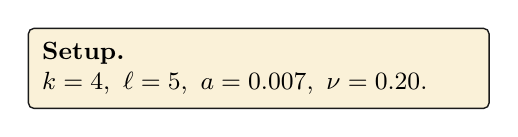
\begin{tikzpicture}
      \node[notecard,text width=5.5cm,align=left] {%
        \textbf{Setup.}\\
        $k=4,\ \ell=5,\ a=0.007,\ \nu=0.20.$
      };
    \end{tikzpicture}
    \end{center}
    \vspace{0.1cm}

    Arrival frequency of carrier 5:
    \[
      f_5^{\rx}=5(1+0.007)+0.20=5.235.
    \]
    Bin 4 sees leftover turns
    \[
      \Delta_{4,5}=f_5^{\rx}-4=1.235.
    \]
    Not an integer $\to$ the loop won't close.
  \end{column}
  \begin{column}{0.49\textwidth}
    Without Doppler:\ $\Delta_{4,5}=1\Rightarrow c_{4,5}=0$.
    \medskip

    With Doppler:
    \[
      c_{4,5}
      =\int_0^1 e^{\jj 2\pi(1.235)t}\,dt
      \approx 0.128+0.117\jj.
    \]
    \[
      |c_{4,5}|\approx 0.173.
    \]
    \begin{center}
    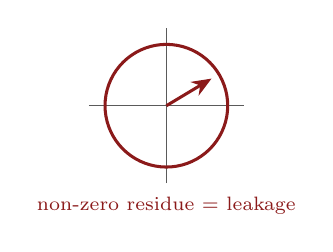
\begin{tikzpicture}[x=0.82cm,y=0.82cm]
      \draw[inkgray] (-1.2,0) -- (1.2,0);
      \draw[inkgray] (0,-1.2) -- (0,1.2);
      \draw[accentred,line width=1.1pt,domain=0:444.6,samples=90]
        plot ({0.95*cos(\x)},{0.95*sin(\x)});
      \draw[flowarr,color=accentred,line width=1.1pt] (0,0) -- (0.70,0.42);
      \node[font=\scriptsize\color{accentred}] at (0,-1.55) {non-zero residue = leakage};
    \end{tikzpicture}
    \end{center}
  \end{column}
\end{columns}
\end{frame}

% =====================================================================
% 3d. From unfinished loop to row term
% =====================================================================
\begin{frame}{From one unfinished loop to one row term}
\stepbadgehdr{3}{$c_{k,\ell}$ is both a loop average and a row multiplier}
\small
\begin{columns}[T,onlytextwidth]
  \begin{column}{0.50\textwidth}
    The received waveform contains \emph{all} carriers at once:
    \[
      r(t)=\sum_{\ell} d_\ell
      e^{\jj 2\pi f_\ell^{\rx}t}+n(t).
    \]
    FFT bin $k$ is a linear averaging machine:
    \[
      y_k=\int_0^1 r(t)e^{-\jj 2\pi kt}\,dt.
    \]
    Substitute the sum into the integral:
    \[
      y_k
      =
      \sum_{\ell} d_\ell
      \underbrace{\int_0^1
      e^{\jj 2\pi(f_\ell^{\rx}-k)t}\,dt}_{\substack{\text{loop average}\\c_{k,\ell}}}
      + n_k .
    \]
  \end{column}
	  \begin{column}{0.48\textwidth}
	    \begin{center}
	    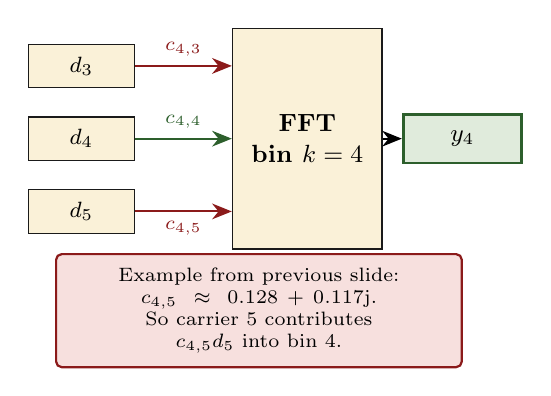
\begin{tikzpicture}[x=0.82cm,y=0.84cm,>=Latex]
	      \node[smallbox,minimum width=1.35cm] (d3) at (-2.55,1.35) {$d_3$};
	      \node[smallbox,minimum width=1.35cm] (d4) at (-2.55,0.25) {$d_4$};
	      \node[smallbox,minimum width=1.35cm] (d5) at (-2.55,-0.85) {$d_5$};

	      \node[draw=ink,fill=paper,line width=0.55pt,align=center,
	        minimum width=1.9cm,minimum height=2.8cm,font=\small\bfseries]
	        (bin) at (0.95,0.25) {FFT\\bin $k=4$};

      \draw[flowarr,color=accentred] (d3) -- node[above,font=\scriptsize] {$c_{4,3}$} (bin.west |- d3);
      \draw[flowarr,color=accentgreen] (d4) -- node[above,font=\scriptsize] {$c_{4,4}$} (bin.west);
      \draw[flowarr,color=accentred] (d5) -- node[below,font=\scriptsize] {$c_{4,5}$} (bin.west |- d5);

	      \node[method,minimum width=1.50cm] (out) at (3.35,0.25) {$y_4$};
	      \draw[flowarr] (bin) -- (out);

	      \node[redcard,text width=4.8cm,font=\scriptsize] at (0.20,-2.35) {%
	        Example from previous slide:\\
	        $c_{4,5}\approx 0.128+0.117\jj$.\\
	        So carrier $5$ contributes $c_{4,5}d_5$ into bin $4$.
	      };
    \end{tikzpicture}
    \end{center}
	  \end{column}
	\end{columns}
	\end{frame}

% =====================================================================
% 3e. Row equation + ICI matrix
% =====================================================================
\begin{frame}{Rows become an ICI matrix}
\stepbadgehdr{3}{stack the row terms and the matrix appears}
\small
\begin{columns}[T,onlytextwidth]
  \begin{column}{0.45\textwidth}
    Clean OFDM:
    \[
      y_k = c_{k,k}\, d_k + n_k,
      \quad
      c_{k,\ell}=0\ \ (\ell\ne k).
    \]
    Doppler OFDM:
    \[
      y_k = c_{k,k}\, d_k
      +\!\!\sum_{\ell\ne k}\!\! c_{k,\ell}\, d_\ell
      + n_k.
    \]
    The off-diagonal terms are \textbf{ICI} — pieces of \emph{other} symbols inside your bin.
    \vspace{0.20cm}
    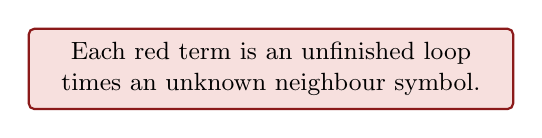
\begin{tikzpicture}
      \node[redcard,text width=5.8cm] {%
        Each red term is an unfinished loop times an unknown neighbour symbol.
      };
    \end{tikzpicture}
  \end{column}
  \begin{column}{0.53\textwidth}
    \begin{center}
    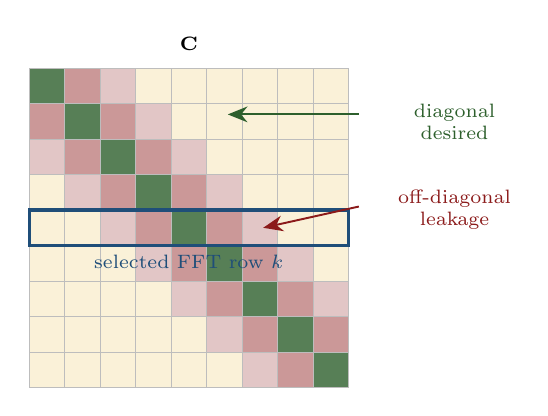
\begin{tikzpicture}[x=0.45cm,y=0.45cm]
      \foreach \r in {0,...,8} {
        \foreach \c in {0,...,8} {
          \pgfmathtruncatemacro{\d}{abs(\r-\c)}
          \ifnum\d=0
            \fill[accentgreen!80] (\c,8-\r) rectangle ++(1,1);
          \else
            \ifnum\d=1
              \fill[accentred!45] (\c,8-\r) rectangle ++(1,1);
            \else
              \ifnum\d=2
                \fill[accentred!25] (\c,8-\r) rectangle ++(1,1);
              \else
                \fill[paper] (\c,8-\r) rectangle ++(1,1);
              \fi
            \fi
          \fi
          \draw[inkgray!40,line width=0.2pt] (\c,8-\r) rectangle ++(1,1);
        }
      }
      \draw[accentblue,line width=1.2pt] (0,4) rectangle (9,5);
      \node[font=\scriptsize\color{accentblue}] at (4.5,3.55) {selected FFT row $k$};
      \node[font=\scriptsize] at (4.5,9.7) {$\mathbf C$};
      \node[font=\scriptsize\color{accentgreen},align=center] at (12.0,7.5)
        {diagonal\\desired};
      \node[font=\scriptsize\color{accentred},align=center] at (12.0,5.0)
        {off-diagonal\\leakage};
      \draw[flowarr,color=accentgreen] (9.3,7.7) -- (5.6,7.7);
      \draw[flowarr,color=accentred] (9.3,5.1) -- (6.6,4.5);
    \end{tikzpicture}
    \end{center}
  \end{column}
\end{columns}
\end{frame}
% =====================================================================
% Final mental model
% =====================================================================
\begin{frame}{Putting it all together}
\stepbadgehdr{$\bigstar$}{the chronological story in one line}
\footnotesize
\begin{center}
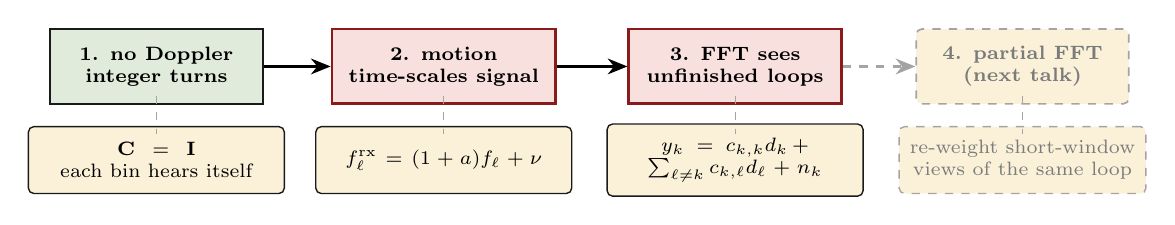
\begin{tikzpicture}[x=1.0cm,y=0.82cm,>=Latex]
  \node[flowbox,minimum width=2.7cm,minimum height=0.95cm,font=\scriptsize\bfseries,fill=grnbg] (a) at (-5.5,0.95)
    {1. no Doppler\\integer turns};
  \node[issue,  minimum width=2.7cm,minimum height=0.95cm,font=\scriptsize\bfseries] (b) at (-1.85,0.95)
    {2. motion\\time-scales signal};
  \node[issue,  minimum width=2.7cm,minimum height=0.95cm,font=\scriptsize\bfseries] (c) at (1.85,0.95)
    {3. FFT sees\\unfinished loops};
  \node[draw=inkgray!55,fill=paper,line width=0.6pt,dashed,rounded corners=2pt,
        align=center,minimum width=2.7cm,minimum height=0.95cm,
        font=\scriptsize\bfseries,text=inkgray!80] (d) at (5.5,0.95)
    {4. partial FFT\\(next talk)};
  \draw[flowarr,line width=1pt] (a) -- (b);
  \draw[flowarr,line width=1pt] (b) -- (c);
  \draw[flowarr,line width=1pt,color=inkgray!55,dashed] (c) -- (d);

  \node[notecard,text width=2.9cm,minimum height=0.85cm,font=\scriptsize] at (-5.5,-0.50)
    {$\mathbf C=\mathbf I$\\\scriptsize each bin hears itself};
  \node[notecard,text width=2.9cm,minimum height=0.85cm,font=\scriptsize] at (-1.85,-0.50)
    {$f_\ell^{\rx}=(1+a)f_\ell+\nu$};
  \node[notecard,text width=2.9cm,minimum height=0.85cm,font=\scriptsize] at (1.85,-0.50)
    {$y_k = c_{k,k}d_k\,+$\\$\sum_{\ell\ne k}c_{k,\ell}d_\ell+n_k$};
  \node[draw=inkgray!55,fill=paper,line width=0.5pt,dashed,rounded corners=2pt,
        align=center,text width=2.9cm,minimum height=0.85cm,
        font=\scriptsize,text=inkgray!80] at (5.5,-0.50)
    {re-weight short-window\\views of the same loop};

  % thin connecting strokes from each row box to its formula card
  \foreach \xpos in {-5.5,-1.85,1.85,5.5} {
    \draw[inkgray!55,line width=0.4pt,dashed] (\xpos,0.50) -- (\xpos,-0.10);
  }
\end{tikzpicture}
\end{center}

\vspace{0.08cm}
\begin{center}
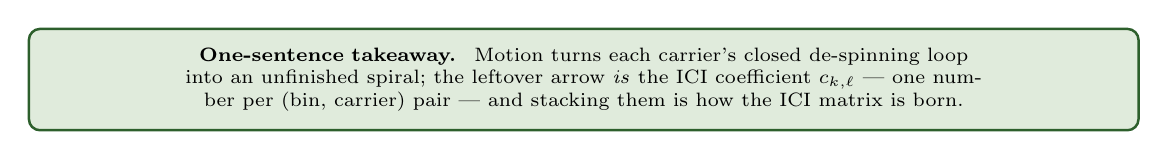
\begin{tikzpicture}
  \node[draw=accentgreen,fill=grnbg,line width=0.9pt,rounded corners=4pt,
        text width=13.6cm,inner sep=7pt,align=center,font=\scriptsize] {%
    \textbf{One-sentence takeaway.}\,\,
    Motion turns each carrier's closed de-spinning loop into an unfinished spiral; the leftover arrow \emph{is} the ICI coefficient $c_{k,\ell}$ --- one number per (bin, carrier) pair --- and stacking them is how the ICI matrix is born.
  };
\end{tikzpicture}
\end{center}

\vspace{0.08cm}
{\scriptsize
\begin{columns}[T,onlytextwidth]
  \begin{column}{0.49\textwidth}
    \textbf{You can now picture}
    \begin{itemize}\setlength{\itemsep}{-0.10em}
      \item a carrier as a clock making $\ell$ turns per symbol,
      \item Doppler as a small fractional spin that ruins closure,
      \item ICI as the leftover arrow from the unfinished loop.
    \end{itemize}
  \end{column}
  \begin{column}{0.49\textwidth}
    \textbf{Next talk: partial FFT (JUNA / RPC)}
    \begin{itemize}\setlength{\itemsep}{-0.10em}
      \item stop the FFT early: keep $M$ short-window views,
      \item weights re-align the wanted arrow, scramble the leaks,
      \item RPC learns weights from pilots; JUNA adds LDPC anchors.
    \end{itemize}
  \end{column}
\end{columns}}

\end{frame}

\end{document}
